\subsection{Схемы телескопов}
Телескопв по своей оптической схеме делятся на 3 типа:
\begin{enumerate}
\item Рефлекторы или диоптрические
\item Рефракторы или катаптрические
\item Катадиоптрические
\end{enumerate}

\textit{Рефлектор} (зеркальный телескоп)~---  оптический телескоп, использующий в качестве светособирающего элемента зеркало.

\textit{Рефрактор} (линзовый телескоп)~---  оптический телескоп, в котором для собирания света используется система линз.

\textit{Катадиоптрический} (зеркально-линзовый) \textit{телескоп}~--- оптический телескоп, в котором используется как система линз, так и зеркал.

Ниже представлены схемы оптических телескопов:


\begin{figure}[h]
\begin{minipage}[h]{0.32\linewidth}
\center{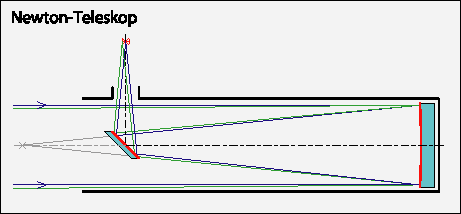
\includegraphics[width=0.67\linewidth]{Newton-Teleskop}}
\end{minipage}
\hfill
\begin{minipage}[h]{0.32\linewidth}
\center{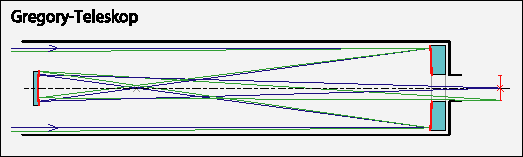
\includegraphics[width=0.6\linewidth]{Gregory-Teleskop}}
\end{minipage}
\hfill
\begin{minipage}[h]{0.32\linewidth}
\center{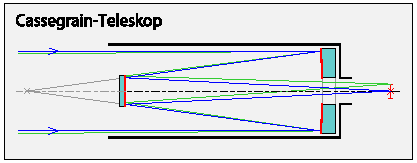
\includegraphics[width=0.6\linewidth]{Cassegrain-Teleskop}}
\end{minipage}
\caption{Рефлекторы}
\end{figure}

\centering
\begin{figure}[!h]
\center{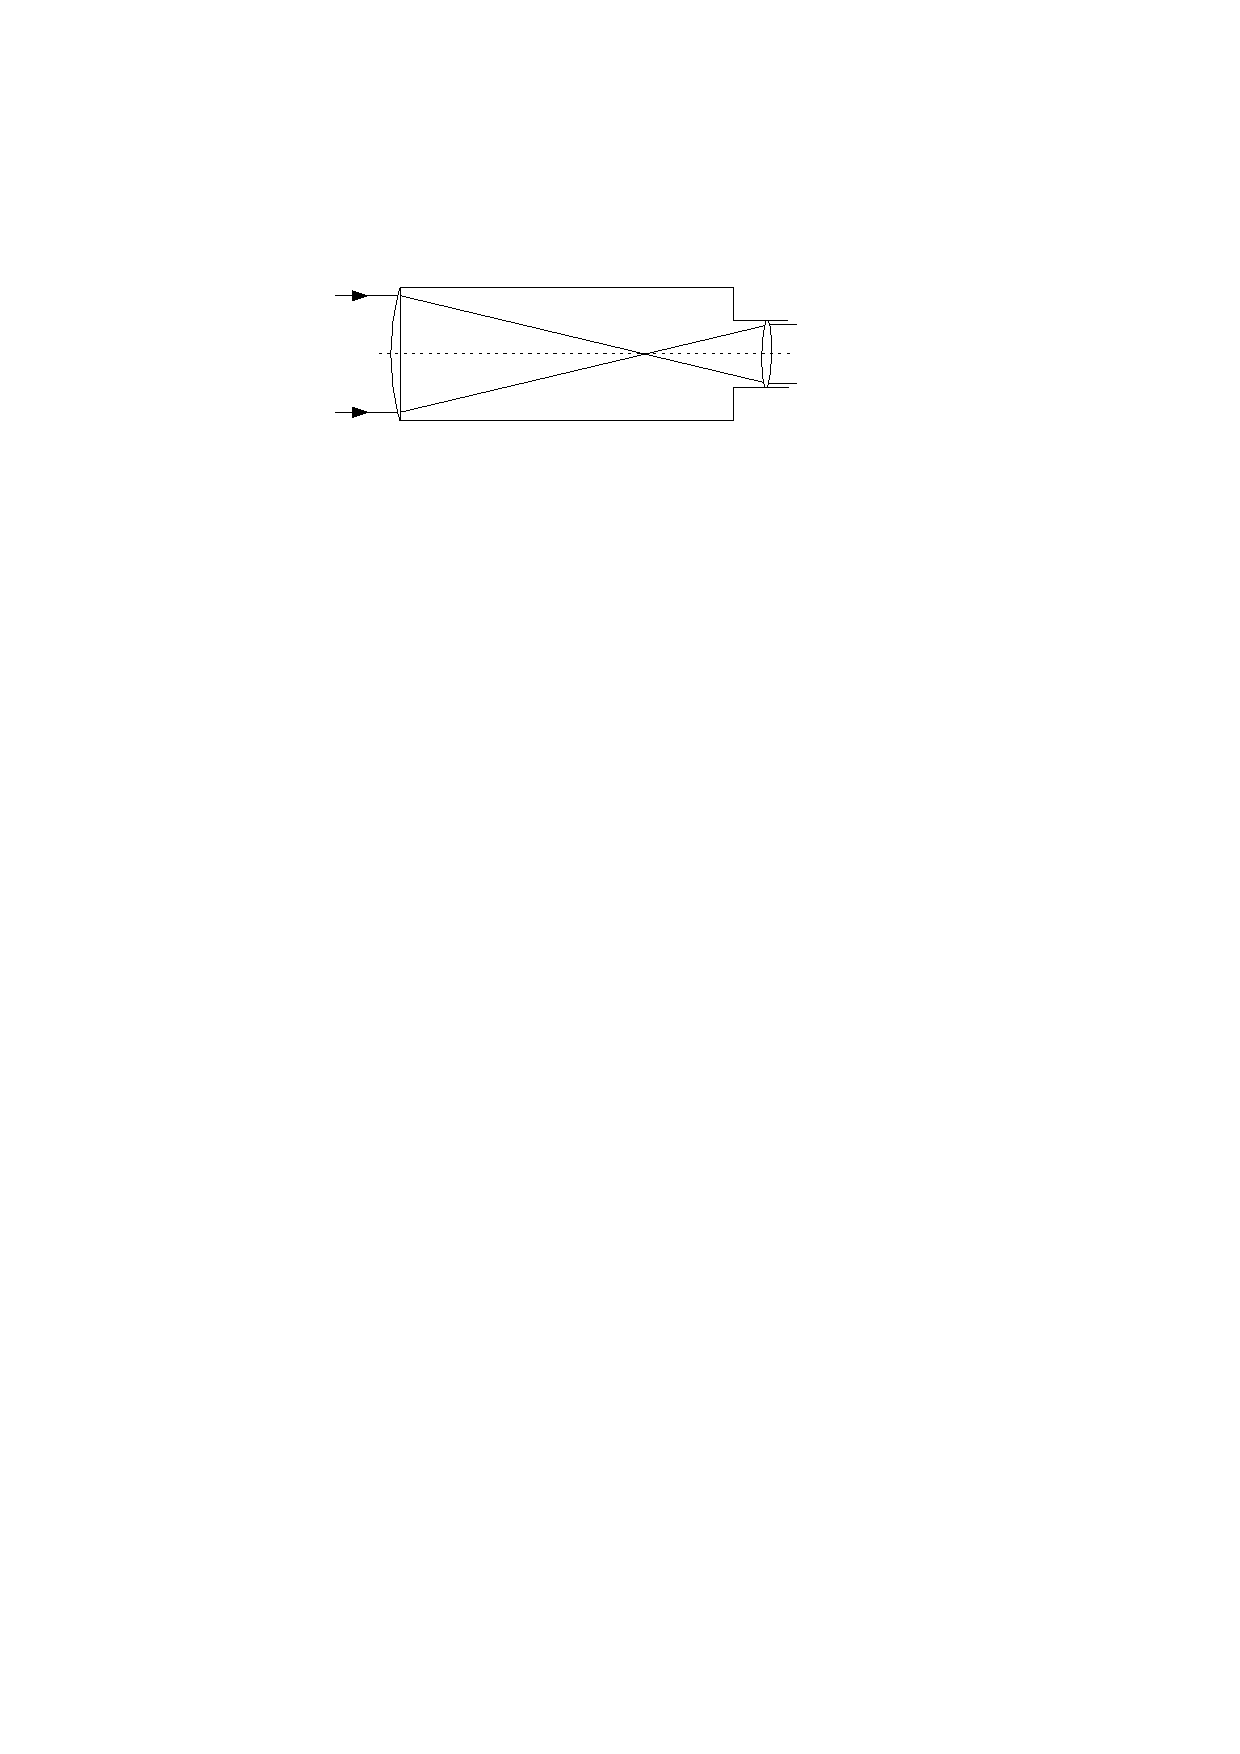
\includegraphics[width=0.6\linewidth]{Refractor}}
\caption{Рефрактор}
\end{figure}